\documentclass[11pt,a4paper]{article}
\usepackage[T1]{fontenc}
\usepackage{lmodern}
\usepackage[top=0.45in, bottom=0.45in, left=0.68in, right=0.68in, headheight=0pt, headsep=0pt]{geometry}
\usepackage{amsmath,amssymb}
\usepackage{xcolor}
\usepackage{tikz}
\usetikzlibrary{arrows.meta,positioning,calc,decorations.pathreplacing}
\usepackage{tcolorbox}
\usepackage{hyperref}
\usepackage{booktabs}
\usepackage{url}
\usepackage{caption}

\hypersetup{
    colorlinks=true,
    linkcolor=blue!70!black,
    citecolor=blue!70!black,
    urlcolor=blue!70!black
}

% Custom Callout Boxes matching math_tools_en / house style
\newtcolorbox{learningobj}{
    colback=blue!3!white,
    colframe=blue!60!black,
    fonttitle=\bfseries\sffamily,
    fontupper=\small,
    title={$\blacktriangleright$ LEARNING OBJECTIVE},
    arc=1.5mm,
    boxrule=0.8pt,
    left=3mm, right=3mm, top=1.2mm, bottom=1.2mm,
    before skip=1mm, after skip=1.5mm
}

\newtcolorbox{groundbreaking}{
    colback=teal!4!white,
    colframe=teal!60!black,
    fonttitle=\bfseries\sffamily,
    fontupper=\small,
    title={$\bigstar$ GROUNDBREAKING FINDING},
    arc=1.5mm,
    boxrule=0.8pt,
    left=3mm, right=3mm, top=1.2mm, bottom=1.2mm,
    before skip=1.5mm, after skip=1mm
}

\newtcolorbox{physicalinsight}{
    colback=yellow!6!white,
    colframe=orange!75!black,
    fonttitle=\bfseries\sffamily,
    fontupper=\small,
    title={$\blacktriangleright$ PHYSICAL INSIGHT},
    arc=1.5mm,
    boxrule=0.8pt,
    left=3mm, right=3mm, top=1.2mm, bottom=1.2mm,
    before skip=1.5mm, after skip=1.5mm
}

\renewcommand{\thefigure}{1.3\alph{figure}}

\begin{document}

% ============================================================================
% PAGE 1: The Probe Wave & Quadrature Projection
% ============================================================================
\vspace*{-4.5mm}
\section*{1.3 Mathematical Modeling: STFT and Mel Filterbank}
\vspace{-2.5mm}

\begin{learningobj}
Rather than memorizing six decoupled DSP formulas, this section deduces each operator from first principles: the probe wave that senses harmonic resonance, the tapering window that kills artificial boundary jumps, the Short-Time Fourier Transform that resolves the Gabor-Heisenberg uncertainty trade-off, the power spectrum that strips superfluous phase, the Mel filterbank that warps linear Hertz to cochlear biology, and the logarithmic compression that mirrors human loudness perception. Every formula is autopsied under our five-beat framework---formula, symbols, physical meaning, hardware price, and what the formula hides---arming the hardware engineer to implement these transforms directly in silicon.
\end{learningobj}

\vspace{1.5mm}
Section 1.2 constructed the physical datapath that packages streaming air pressure into discrete frames. Section 1.3 is the mathematical microscope placed over a single packet, deducing each spectral operator from wave interference and auditory perception.

\vspace{-1mm}
\subsection*{1. The Probe Wave: Orthogonal Quadrature Projection}
\vspace{-2mm}

Before writing down the Fourier summation, consider the physical interrogation problem. An unknown acoustic packet arrives at the sensor as a discrete sequence of air-pressure displacements $x_\ell[n]$. How does a computational circuit determine whether this packet vibrates at a specific frequency $f_k$?

In classical physics, resonance is detected by probing: we bring an external oscillator of known frequency $\omega_k$ into contact with the system and observe steady-state energy transfer. In digital computation, we generate an internal reference probe tone and evaluate its interference against the incoming signal through an inner product: $\int_0^T x(t) \cos(\omega_k t) \, dt$. If $x(t)$ contains an oscillation at $\omega_k$ in identical phase ($\cos(\omega_k t)$), the product becomes $\cos^2(\omega_k t) = \frac{1 + \cos(2\omega_k t)}{2}$. Integrated across $T$, the $2\omega_k$ harmonic averages to zero, leaving a positive DC accumulation of $\frac{T}{2}$. If $x(t)$ oscillates at any different harmonic $\omega_m$ ($m \ne k$), the cross-product integrates to identically zero. The probe resonates exclusively with its own frequency.

Now expose the fatal flaw of a single probe wave: \textbf{phase blindness}. If the incoming packet arrives delayed by a quarter-cycle (a phase shift of $\pi/2$, turning the input into a pure sine wave $\sin(\omega_k t)$), the product evaluated by our cosine probe becomes $\sin(\omega_k t)\cos(\omega_k t) = \frac{1}{2}\sin(2\omega_k t)$. Over the integration interval $T$, this wave integrates to exactly zero: $\int_0^T \sin(\omega_k t) \cos(\omega_k t) \, dt = 0$. The single probe reports zero energy. A pure acoustic tone is roaring through the physical transducer, but because it arrived with a $90^\circ$ phase offset, our mathematical detector is completely deaf to it.

To eliminate phase blindness, we must interrogate the incoming wave with \textbf{two orthogonal probes in quadrature}: an in-phase probe oscillating as $\cos(\omega_k t)$ and a quadrature probe oscillating as $-\sin(\omega_k t)$ (delayed by $90^\circ$). When an arbitrary signal $x(t) = A \cos(\omega_k t + \theta)$ strikes this dual-branch detector, the cosine branch measures $A \cos\theta$ and the sine branch measures $A \sin\theta$. By the Pythagorean theorem, total signal magnitude is recovered with absolute phase immunity: $A = \sqrt{(A\cos\theta)^2 + (A\sin\theta)^2}$. Euler's identity, $e^{-j\phi} = \cos\phi - j\sin\phi$, is the algebraic packaging of this two-channel physical quadrature receiver.

\vspace{-4mm}
\begin{center}
\begin{minipage}{\textwidth}
\centering
\scalebox{0.62}{\input{chapter01/fig_1_3a.tex}}\\[0.5mm]
\begin{minipage}{0.96\textwidth}
\small\textbf{Figure 1.3a}: \textbf{Probe-wave quadrature interferometer.} (1)~\textbf{What it is:} The internal architecture of a single Fourier frequency bin evaluated as a dual-branch correlation receiver. (2)~\textbf{What to look at:} The incoming frame $x_\ell[n]$ splits into parallel branches multiplied by $\cos(2\pi kn/N)$ (in-phase) and $-\sin(2\pi kn/N)$ (quadrature), accumulating into real and imaginary coordinates. (3)~\textbf{What it proves:} Complex numbers in spectral analysis are not imaginary quantities; they represent the two physical orthogonal axes required to measure wave energy independently of arrival phase.
\end{minipage}
\end{minipage}
\end{center}
\vspace{-4mm}

\begin{groundbreaking}
A complex exponential in digital signal processing is neither an abstract mathematical convenience nor imaginary physics. It is a dual-channel hardware quadrature receiver: two orthogonal reference oscillators ($\cos$ and $-\sin$) beating against the incoming pressure wave, recovering acoustic magnitude with absolute invariance to arrival phase.
\end{groundbreaking}

\clearpage

% ============================================================================
% PAGE 2: Autopsy 1 & Autopsy 2 (Windowing + Figure 6)
% ============================================================================
\vspace*{-4.5mm}
\subsubsection*{The 5-Beat Autopsy: The Probe Wave}
\vspace{-2mm}
{\small
\textbf{Beat 1: The Formula.} $X_\ell[k] = \sum_{n=0}^{N-1} x_\ell[n] \, e^{-j \frac{2\pi k n}{N}} = \sum_{n=0}^{N-1} x_\ell[n] \cos\left(\frac{2\pi k n}{N}\right) - j \sum_{n=0}^{N-1} x_\ell[n] \sin\left(\frac{2\pi k n}{N}\right)$\\[1mm]
\textbf{Beat 2: The Symbols.} $k \in \{0, \dots, N-1\}$ is the discrete frequency bin ($f_k = k \frac{f_s}{N} = k \times 31.25\text{ Hz}$ for $N=512, f_s=16\text{ kHz}$); $n \in \{0, \dots, N-1\}$ is the discrete sample index; $x_\ell[n]$ is the $\ell$-th framed signal; $j = \sqrt{-1}$ represents the $90^\circ$ quadrature rotation; $X_\ell[k] \in \mathbb{C}$ is the complex spectral coefficient.\\[1mm]
\textbf{Beat 3: The Physical Meaning.} Quadrature projection measures total acoustic energy residing at frequency $f_k$. The real component gauges correlation with a pure cosine, while the imaginary component gauges correlation with a negative sine. Euclidean magnitude $|X_\ell[k]| = \sqrt{\text{Re}^2 + \text{Im}^2}$ recovers total signal amplitude invariant to phase delay $\theta = \operatorname{atan2}(\text{Im}, \text{Re})$.\\[1mm]
\textbf{Beat 4: The Hardware Price.} Evaluating $N$ bins via naive DFT requires $N^2 = 512^2 = 262{,}144$ complex MACs ($1{,}048{,}576$ real ops) per frame ($104.9\text{ MFLOPS}$ at $100\text{ fps}$). Cooley-Tukey FFT collapses complexity to $\frac{N}{2}\log_2 N = 256 \times 9 = 2{,}304$ complex MACs ($9{,}216$ real ops)---a $113.8\times$ arithmetic reduction.\\[1mm]
\textbf{Beat 5: What the Formula Does Not Say.} The summation presumes periodic repetition ($x[n] = x[n+N]$). If endpoints $x[0]$ and $x[N-1]$ mismatch, the step discontinuity injects artificial high-frequency energy across all $N$ bins (\textbf{spectral leakage}), corrupting the spectrum unless tempered by windowing.
}

\vspace{1mm}
\hrule
\vspace{1mm}

\subsection*{2. The Windowed Frame: Tempering Boundary Discontinuities}
\vspace{-2mm}
To eliminate the boundary step discontinuity, the raw audio packet is tapered smoothly toward zero before projection.

\subsubsection*{The 5-Beat Autopsy: The Windowed Frame}
\vspace{-2mm}
{\small
\textbf{Beat 1: The Formula.} $\tilde{x}_\ell[n] = x_\ell[n] \cdot w[n], \; w[n] = 0.54 - 0.46 \cos\left(\frac{2\pi n}{L-1}\right) \; (0 \le n < L); \quad \tilde{x}_\ell[n] = 0 \; (L \le n < N)$\\[1mm]
\textbf{Beat 2: The Symbols.} $x_\ell[n]$ is the raw frame from the ring buffer ($L = 400$ samples, $25\text{ ms}$ at $16\text{ kHz}$); $w[n]$ is the Hamming window; $\tilde{x}_\ell[n]$ is the zero-padded sequence ($N = 512$ points); $L$ sets physical window resolution $\Delta f_{\text{window}} \approx 40\text{ Hz}$; $N$ sets FFT grid resolution $\Delta f_{\text{bin}} = 31.25\text{ Hz}$.\\[1mm]
\textbf{Beat 3: The Physical Meaning.} Slicing rectangularly convolves the spectrum with a sinc function whose side-lobes decay at only $-6\text{ dB/octave}$ (first side-lobe at $-13\text{ dB}$). The raised-cosine Hamming window tapers boundaries to $w[0] = w[L-1] = 0.08$, suppressing the first side-lobe to $-44\text{ dB}$ ($31\text{ dB}$ leakage reduction).\\[1mm]
\textbf{Beat 4: The Hardware Price.} Requires $L = 400$ real multiplications per frame. Exploiting symmetry ($w[n] = w[L-1-n]$), coefficients fold into a $200$-entry 16-bit lookup table ($400$ bytes, half a BRAM-18K). Pipelined through a single DSP48 slice, all multiplications complete in $400$ clock cycles ($4.0\ \mu\text{s}$ at $100\text{ MHz}$).\\[1mm]
\textbf{Beat 5: What the Formula Does Not Say.} Windowing destroys signal energy (coherent gain $\approx 0.54$, noise power gain $\approx 0.397$, an attenuation of $1.58\text{ dB}$). Edge samples are attenuated near zero. To prevent blind spots, consecutive frames overlap heavily: hop size $H = 160$ ($10\text{ ms}$) creates a $60\%$ overlap ($240$ shared samples), restoring uniform cumulative coverage.
}

\vspace{-3.5mm}
\begin{center}
\begin{minipage}{\textwidth}
\centering
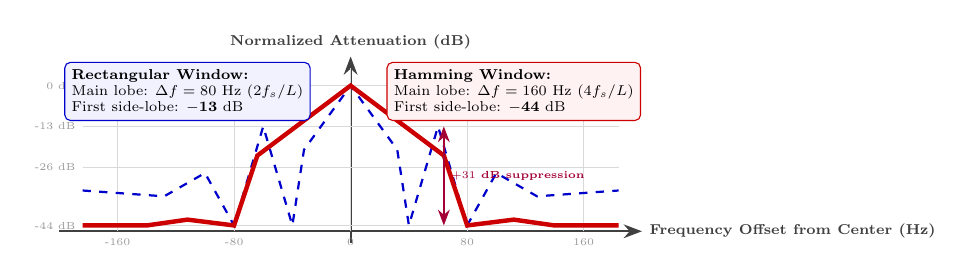
\begin{tikzpicture}[>=Stealth, scale=0.74, every node/.style={transform shape}, font=\small]
  % Grid and Axes
  \draw[->, black!75, thick] (-5.0, -2.5) -- (5.0, -2.5) node[right, font=\scriptsize\bfseries] {Frequency Offset from Center (Hz)};
  \draw[->, black!75, thick] (0, -2.7) -- (0, 0.5) node[above, font=\scriptsize\bfseries] {Normalized Attenuation (dB)};

  \foreach \y/\lbl in {0/{0}, -0.7/{-13}, -1.4/{-26}, -2.4/{-44}} {
    \draw[gray!30, thin] (-4.6, \y) -- (4.6, \y);
    \node[left, font=\tiny, text=gray!80] at (-4.6, \y) {\lbl~dB};
  }
  \foreach \x/\lbl in {-4/{-160}, -2/{-80}, 0/{0}, 2/{80}, 4/{160}} {
    \draw[gray!30, thin] (\x, -2.5) -- (\x, 0.3);
    \node[below, font=\tiny, text=gray!80] at (\x, -2.5) {\lbl};
  }

  % Rectangular window spectrum (sinc shape, blue dashed)
  \draw[blue!80!black, thick, dashed] 
    (-4.6, -1.8) -- (-3.2, -1.9) -- (-2.5, -1.5) -- (-2.0, -2.4) 
    -- (-1.5, -0.7) -- (-1.0, -2.4) -- (-0.8, -1.1) -- (0, 0) 
    -- (0.8, -1.1) -- (1.0, -2.4) -- (1.5, -0.7) -- (2.0, -2.4) 
    -- (2.5, -1.5) -- (3.2, -1.9) -- (4.6, -1.8);

  % Hamming window spectrum (broader main lobe, heavily suppressed side lobes, red solid)
  \draw[red!80!black, ultra thick] 
    (-4.6, -2.4) -- (-3.5, -2.4) -- (-2.8, -2.3) -- (-2.0, -2.4) 
    -- (-1.6, -1.2) -- (0, 0) -- (1.6, -1.2) -- (2.0, -2.4) 
    -- (2.8, -2.3) -- (3.5, -2.4) -- (4.6, -2.4);

  % Annotations
  \node[draw=blue!80!black, fill=blue!5, rounded corners=2pt, font=\scriptsize, align=left] at (-2.8, -0.1) {
    \textbf{Rectangular Window:}\\
    Main lobe: $\Delta f = 80\text{ Hz}$ ($2f_s/L$)\\
    First side-lobe: $\mathbf{-13\text{ dB}}$
  };

  \node[draw=red!80!black, fill=red!5, rounded corners=2pt, font=\scriptsize, align=left] at (2.8, -0.1) {
    \textbf{Hamming Window:}\\
    Main lobe: $\Delta f = 160\text{ Hz}$ ($4f_s/L$)\\
    First side-lobe: $\mathbf{-44\text{ dB}}$
  };

  \draw[<->, purple!85!black, semithick] (1.6, -0.7) -- (1.6, -2.4) node[midway, right, font=\tiny\bfseries] {$+31\text{ dB}$ suppression};
\end{tikzpicture}\\[1mm]
\begin{minipage}{0.96\textwidth}
\small\textbf{Figure 6}: \textbf{Spectral leakage: Rectangular vs.\ Hamming window ($L = 400$, $f_s = 16\text{ kHz}$).} (1)~\textbf{What it is:} Transfer functions for rectangular versus Hamming windowing. (2)~\textbf{What to look at:} Main lobe doubles in width ($80\text{ Hz} \to 160\text{ Hz}$), but the first side-lobe drops from $-13\text{ dB}$ to $-44\text{ dB}$ ($31\text{ dB}$ suppression). (3)~\textbf{What it proves:} Windowing trades frequency sharpness for dynamic range, preventing loud formants from masking quiet consonant harmonics.
\end{minipage}
\end{minipage}
\end{center}
\vspace{-3.5mm}

\begin{physicalinsight}
Windowing is an unavoidable bargain with the uncertainty principle: we accept a doubling of main-lobe width (from $80\text{ Hz}$ to $160\text{ Hz}$) to buy $31\text{ dB}$ of side-lobe suppression. Without this suppression, the fundamental harmonic of an adult male voice ($120\text{ Hz}$) would wash out quiet sibilant formants ($3\text{ kHz}$) across the entire register.
\end{physicalinsight}

\clearpage

% ============================================================================
% PAGE 3: Autopsy 3 (STFT) & Autopsy 4 (Power Spectrum)
% ============================================================================
\vspace*{-4.5mm}
\subsection*{3. The Short-Time Fourier Transform (STFT)}
\vspace{-2mm}
Having windowed and zero-padded the frame, we assemble the time-dependent spectral matrix that maps phonetic transitions as they evolve through time.

\subsubsection*{The 5-Beat Autopsy: The Short-Time Fourier Transform}
\vspace{-2mm}
{\small
\textbf{Beat 1: The Formula.} $X[\ell, k] = \sum_{n=0}^{N-1} \tilde{x}_\ell[n] \, e^{-j \frac{2\pi k n}{N}} = \sum_{n=0}^{L-1} x[\ell H + n] \, w[n] \, e^{-j \frac{2\pi k n}{N}} \quad \left(0 \le k \le \frac{N}{2}\right)$\\[1mm]
\textbf{Beat 2: The Symbols.} $\ell \in \mathbb{Z}$ is the temporal frame index, advancing in strides of hop size $H = 160$ samples ($10\text{ ms}$ at $16\text{ kHz}$); $k \in \{0, 1, \dots, N/2\}$ is the frequency bin index. Because the input signal $x[n]$ is real-valued, the negative frequency spectrum is conjugate-symmetric ($X[\ell, N-k] = X^*[\ell, k]$), allowing us to discard the redundant upper half and retain exactly $N/2 + 1 = 257$ unique frequency bins ($0 \le k \le 256$); $H = 160$ sets the frame rate $f_{\text{frame}} = f_s / H = 100\text{ Hz}$.\\[1mm]
\textbf{Beat 3: The Physical Meaning.} The STFT transforms a 1D time-series into a 2D complex time-frequency coordinate space (the complex spectrogram). It freezes the vibrating human vocal tract into stationary $25\text{ ms}$ acoustic snapshots, resolving the Gabor-Heisenberg uncertainty trade-off ($\Delta t \cdot \Delta f \ge \frac{1}{4\pi}$): temporal resolution is held at $25\text{ ms}$ (fine enough to isolate rapid stop bursts), while frequency resolution is held at $40\text{ Hz}$ (sharp enough to distinguish individual vowel formants).\\[1mm]
\textbf{Beat 4: The Hardware Price.} On FPGA hardware, the STFT is implemented via a pipelined radix-2 Cooley-Tukey engine. For $N = 512$, the architecture comprises $\log_2(512) = 9$ cascaded stages. Each stage executes $N/2 = 256$ butterfly operations ($A' = A + W_N^r B, \; B' = A - W_N^r B$), requiring 1 complex multiplication (4 real DSP multipliers, 2 real adders) and 2 complex additions per butterfly. Pipelining all 9 stages in hardware consumes 36 DSP48 slices and processes continuous streaming frames at full clock rate without stalling the incoming audio stream.\\[1mm]
\textbf{Beat 5: What the Formula Does Not Say.} Zero-padding from $L = 400$ to $N = 512$ does not improve the physical frequency resolution of the audio. Padding merely interpolates the discrete Fourier transform more densely along the frequency axis (sampling at $31.25\text{ Hz}$ intervals instead of $40\text{ Hz}$). The true resolving power remains fundamentally bounded by the $25\text{ ms}$ window length ($40\text{ Hz}$). Two pure tones separated by only $15\text{ Hz}$ remain blurred together, regardless of whether $N$ is padded to $512$ or $65{,}536$ points.
}

\vspace{1.5mm}
\hrule
\vspace{1.5mm}

\subsection*{4. The Power Spectrum: Magnitude Squared}
\vspace{-2mm}
Downstream acoustic models do not ingest raw complex coordinates. We must convert the complex spectral bins into real-valued acoustic energy.

\subsubsection*{The 5-Beat Autopsy: The Power Spectrum}
\vspace{-2mm}
{\small
\textbf{Beat 1: The Formula.} $P[\ell, k] = \frac{1}{N} |X[\ell, k]|^2 = \frac{1}{N} \left( \text{Re}(X[\ell, k])^2 + \text{Im}(X[\ell, k])^2 \right) \quad \left(0 \le k \le \frac{N}{2}\right)$\\[1mm]
\textbf{Beat 2: The Symbols.} $P[\ell, k] \in \mathbb{R}_{\ge 0}$ is the power spectral density at frame $\ell$ and frequency bin $k$, representing acoustic power per frequency bin (shape: $[1, 257]$); $\text{Re}(X[\ell, k])$ and $\text{Im}(X[\ell, k])$ are the real and imaginary components from the STFT; $1/N = 1/512 \approx 1.953 \times 10^{-3}$ is the Parseval energy normalization constant.\\[1mm]
\textbf{Beat 3: The Physical Meaning.} Computes the Euclidean squared magnitude of each complex bin vector, discarding phase angle $\theta[\ell, k] = \operatorname{atan2}(\text{Im}, \text{Re})$. Under Ohm's acoustical law, human speech perception is largely phase-deaf: the auditory cortex identifies phonemes primarily by tracking the resonant energy peaks (formants) produced by vocal tract geometry, independent of relative harmonic phase offsets.\\[1mm]
\textbf{Beat 4: The Hardware Price.} For each 257-bin frame, computing $P[\ell, k]$ requires $257 \times 2 = 514$ real squarings, $257$ real additions, and $257$ constant scalings. On FPGA, this maps onto 2 DSP48 slices operating in parallel across 257 clock cycles ($2.57\ \mu\text{s}$ at $100\text{ MHz}$). Crucially, computing power ($|X|^2$) rather than magnitude ($|X|$) avoids the hardware square root operation entirely, saving thousands of logic gates and multi-cycle CORDIC pipelines.\\[1mm]
\textbf{Beat 5: What the Formula Does Not Say.} Discarding phase is mathematically irreversible. Without phase, exact time-domain signal reconstruction is impossible; reconstructing intelligible audio from $P[\ell, k]$ requires iterative heuristic phase estimation (the Griffin-Lim algorithm) or a deep neural vocoder. For speech recognition and keyword spotting, discarding phase is an intentional noise-reduction feature; for speech separation or echo cancellation, however, phase distortion severely degrades perceived audio quality.
}

\clearpage

% ============================================================================
% PAGE 4: Autopsy 5 (Mel Filterbank) + Figure 1.3b
% ============================================================================
\vspace*{-4.5mm}
\subsection*{5. The Mel Filterbank: Perceptual Warp \& Non-Uniform Integration}
\vspace{-2mm}
Linear frequency bins ($0, 31.25, \dots, 8{,}000\text{ Hz}$) treat all frequencies with uniform numerical weight. Human hearing, however, perceives pitch logarithmically. To align spectral features with biological cochlear mechanics, we map linear frequency $f$ to the perceptual \textbf{Mel scale} (Stevens et al., 1937; O'Shaughnessy, 1987): $m = \text{mel}(f) = 2595 \log_{10}(1 + f/700) = 1127 \ln(1 + f/700) \iff f = 700 (10^{m/2595} - 1)$. Across our $0\text{--}8{,}000\text{ Hz}$ band, the Mel range spans $0$ to $2840.02\text{ Mels}$. Dividing this interval into $M = 80$ uniform bands with $M+2 = 82$ edge points ($\Delta m \approx 35.06\text{ Mels}$) and rounding to FFT bins yields the non-linear filter centers $f_{\text{bin}}[m]$.

\subsubsection*{The 5-Beat Autopsy: The Mel Filterbank}
\vspace{-2mm}
{\small
\textbf{Beat 1: The Formula.} $S[\ell, m] = \sum_{k=0}^{N/2} W[m, k] \cdot P[\ell, k] \; (0 \le m < M)$, where $W[m, k]$ is defined by triangular slopes: $\frac{k - f_{\text{bin}}[m-1]}{f_{\text{bin}}[m] - f_{\text{bin}}[m-1]}$ for $k \in [f_{\text{bin}}[m-1], f_{\text{bin}}[m]]$ and $\frac{f_{\text{bin}}[m+1] - k}{f_{\text{bin}}[m+1] - f_{\text{bin}}[m]}$ for $k \in [f_{\text{bin}}[m], f_{\text{bin}}[m+1]]$.\\[0.8mm]
\textbf{Beat 2: The Symbols.} $m \in \{0, \dots, 79\}$ is the Mel filter index ($M = 80$); $W \in \mathbb{R}^{80 \times 257}$ is the triangular filterbank matrix; $f_{\text{bin}}[m]$ is the discrete FFT center bin; $S[\ell, m]$ is the Mel spectral energy vector (shape: $[1, 80]$).\\[0.8mm]
\textbf{Beat 3: The Physical Meaning.} Implements the tonotopic organization of the human cochlea. The stiff basilar membrane base resonates with high frequencies over broad regions, while the flexible apex resonates with low frequencies over narrow bands. Pooling 257 linear bins into 80 Mel bands matches biological perception and compresses feature dimensionality by $68.9\%$.\\[0.8mm]
\textbf{Beat 4: The Hardware Price.} Dense matrix multiplication requires $80 \times 257 = 20{,}560$ MACs per frame. However, $W$ is extraordinarily sparse: over $90\%$ of entries are zero. Because adjacent filters overlap by $50\%$ and partition unity ($\sum_m W[m, k] = 1$), each linear FFT bin $k$ contributes to at most two Mel bands. Storing the filterbank as a sparse table of start/stop indices and slopes reduces arithmetic workload from $20{,}560$ MACs down to exactly $514$ MACs per frame.\\[0.8mm]
\textbf{Beat 5: What the Formula Does Not Say.} The discretization collapse trap! On a finite digital grid ($N = 512, f_s = 16\text{ kHz}, \Delta f = 31.25\text{ Hz}$), low-frequency filter bandwidths are narrower than the FFT bin spacing. When continuous centers round to integer bins, adjacent centers can snap to the exact same bin ($f_{\text{bin}}[m-1] = f_{\text{bin}}[m]$). In our reference pipeline \nolinkurl{chapter01/exp_01_streaming_audio_pipeline.py}, Band 2 collapses, yielding an empty filter that outputs zero energy. Hardware implementations must enforce an explicit minimum bandwidth floor ($\ge 1$ bin) to prevent dead Mel channels.
}

\vspace{-4mm}
\begin{center}
\begin{minipage}{\textwidth}
\centering
\scalebox{0.70}{\input{chapter01/fig_1_3b.tex}}\\[0.8mm]
\begin{minipage}{0.96\textwidth}
\small\textbf{Figure 1.3b}: \textbf{257 linear FFT bins collapsing under 80 Mel triangular filters.} (1)~\textbf{What it is:} Architectural mapping of 257 linear frequency bins ($0\text{--}8{,}000\text{ Hz}$) into 80 perceptual Mel triangular filters. (2)~\textbf{What to look at:} In region (a), low filters are dense and narrow, while high filters expand exponentially. In region (b), Band $m=0$ integrates only 3 bins, whereas Band $m=79$ pools 45 bins ($6{,}593\text{--}8{,}000\text{ Hz}$). (3)~\textbf{What it proves:} The filterbank concentrates spectral resolution in phonetic formant bands while drastically reducing input dimensionality for downstream neural networks.
\end{minipage}
\end{minipage}
\end{center}
\vspace{-4mm}

\begin{physicalinsight}
The Mel filterbank is not merely dimensionality reduction ($257 \to 80$); it is an unequal information concentrator. In the low frequencies ($0\text{--}1\text{ kHz}$), where pitch and the first two vowel formants reside, each Mel band integrates only 1 to 3 FFT bins, preserving fine harmonic detail. In the high frequencies ($6\text{--}8\text{ kHz}$), where voiceless fricatives spread diffuse noise, a single Mel band pools over 40 FFT bins. It discards superfluous high-frequency harmonic granularity while preserving overall spectral envelope.
\end{physicalinsight}

\clearpage

% ============================================================================
% PAGE 5: Autopsy 6 (Log Compression) & The Silicon Reality Check
% ============================================================================
\vspace*{-4.5mm}
\subsection*{6. Logarithmic Energy Compression: Decibel Auditory Dynamic Range}
\vspace{-2mm}
The final transformation compresses wide physical energy variations into a normalized feature space suitable for neural network layers.

\subsubsection*{The 5-Beat Autopsy: Logarithmic Compression}
\vspace{-2mm}
{\small
\textbf{Beat 1: The Formula.} $F[\ell, m] = \ln\left( \max(S[\ell, m], \epsilon) \right) \quad \text{or} \quad \log_{10}\left( S[\ell, m] + \epsilon \right) \quad (0 \le m < M)$\\[1mm]
\textbf{Beat 2: The Symbols.} $F[\ell, m] \in \mathbb{R}$ is the log-Mel filterbank energy feature (shape: $[1, 80]$); $S[\ell, m]$ is the raw Mel band energy from Transform 5; $\epsilon = 10^{-10}$ (floating-point floor) or $\epsilon = 2^{-16}$ (fixed-point floor) prevents catastrophic $\log(0) \to -\infty$ evaluation during silence or digital zero inputs.\\[1mm]
\textbf{Beat 3: The Physical Meaning.} Implements the Weber-Fechner law of human perception: perceived sound loudness scales logarithmically with acoustic power across a dynamic range exceeding $100\text{ dB}$ ($10^{10}$ in physical energy). Furthermore, the logarithm separates multiplicative acoustic effects into additive terms:
$y(t) = s(t) * h(t) \implies |Y(f)| \approx |S(f)| \cdot |H(f)| \implies \log |Y| \approx \log |S| + \log |H|$. Microphone frequency response and room reverberation $H(f)$ become simple constant additive offsets, allowing Cepstral Mean Subtraction (CMN) to remove channel distortion using simple linear subtraction.\\[1mm]
\textbf{Beat 4: The Hardware Price.} On GPUs, computing $\ln(x)$ executes in a single cycle using Special Function Units (SFUs) via \texttt{\_\_logf()}. On FPGAs, floating-point natural logarithm logic is expensive and introduces variable latency. In hardware, logarithm is transformed to base-2: $\ln(x) = \ln(2) \cdot \log_2(x) \approx 0.693147 \cdot (E + \text{mantissa\_lut})$. A hardware priority encoder extracts the exponent $E$ in 1 clock cycle by counting leading zeros, while the fractional mantissa is interpolated from a 64-entry piecewise linear lookup table. This provides full precision with 0 DSP slices and deterministic 1-cycle latency.\\[1mm]
\textbf{Beat 5: What the Formula Does Not Say.} The logarithm acts as an extreme dynamic range expander near zero: $\frac{d}{dx}\ln(x) = \frac{1}{x} \to \infty$ as $x \to 0$. Tiny background noise variations between $10^{-6}$ and $10^{-8}$ produce enormous $-4.6$ swings in log-Mel feature space, whereas identical absolute fluctuations at signal level $1.0$ produce negligible change. Setting $\epsilon$ too small ($10^{-20}$) creates massive negative outliers that destroy 8-bit integer quantization (INT8) scales and destabilize neural network gradient descent.
}

\vspace{2mm}
\hrule
\vspace{2mm}

\subsection*{The Silicon Reality Check: Bridge to Section 1.4}

The mathematical derivations of STFT and Mel filterbanks in this section assume infinite-precision real arithmetic, zero-latency random access to memory, and instantaneous matrix operations. But silicon does not compute on infinite fields. When these six equations are implemented on edge hardware---whether the massively parallel Single-Instruction Multiple-Threads (SIMT) streaming multiprocessors of NVIDIA's Jetson Orin or the spatially configured pipeline registers and Block RAMs of AMD's Zynq UltraScale+ FPGA---the abstract mathematics collides violently with memory bandwidth saturation, L2 cache thrashing, fixed-point rounding noise, and kernel launch overheads.

In Section 1.4, we leave the blackboard behind and confront the silicon reality: profiling the exact latency bottlenecks, memory footprints, and architectural fractures of executing streaming Mel features on real edge hardware.

\vspace{2.5mm}
\begin{center}
\begin{tcolorbox}[colback=gray!5!white, colframe=gray!60!black, arc=1.5mm, boxrule=0.6pt, width=0.96\linewidth, left=3mm, right=3mm, top=1.2mm, bottom=1.2mm]
\small\textbf{Summary of Mathematical Transformations in the Edge Voice Frontend}
\begin{itemize}\setlength{\itemsep}{-0.5pt}\setlength{\parsep}{0pt}\setlength{\topsep}{1pt}
    \item \textbf{Probe Wave Projection:} Interrogates input wave with orthogonal quadrature reference oscillators ($\cos$, $-\sin$), extracting in-phase and quadrature coordinates with phase invariance ($N=512$).
    \item \textbf{Windowed Frame:} Tapers $L=400$ samples with a Hamming raised-cosine profile, suppressing boundary side-lobes by $31\text{ dB}$ (from $-13\text{ dB}$ to $-44\text{ dB}$) at the cost of doubling main-lobe width ($80\text{ Hz} \to 160\text{ Hz}$).
    \item \textbf{STFT:} Resolves Gabor-Heisenberg time-frequency trade-off at $25\text{ ms} / 40\text{ Hz}$, generating 257 non-redundant complex frequency bins at a $10\text{ ms}$ cadence.
    \item \textbf{Power Spectrum:} Discards perceptual phase to extract real-valued energy ($P = \frac{1}{N}|X|^2$), avoiding square-root logic in silicon.
    \item \textbf{Mel Filterbank:} Pools 257 linear bins into 80 biological cochlear bands ($68.9\%$ compression), reducing sparse hardware MACs from $20{,}560$ to $514$.
    \item \textbf{Log Compression:} Compresses dynamic range over $100\text{ dB}$ via Weber-Fechner mapping, converting multiplicative acoustic channel coloration into additive offsets.
\end{itemize}
\end{tcolorbox}
\end{center}

\end{document}
